\documentclass[a4paper]{article}
\usepackage[pdftex]{hyperref}
\usepackage[latin1]{inputenc}
\usepackage[english]{babel}
\usepackage{a4wide}
\usepackage{amsmath}
\usepackage{amssymb}
\usepackage{algorithmic}
\usepackage{algorithm}
\usepackage{ifthen}
\usepackage{listings}
% move the asterisk at the right position
\lstset{basicstyle=\ttfamily,tabsize=4,literate={*}{${}^*{}$}1}
%\lstset{language=C,basicstyle=\ttfamily}
\usepackage{moreverb}
\usepackage{palatino}
\usepackage{multicol}
\usepackage{tabularx}
\usepackage{comment}
\usepackage{verbatim}
\usepackage{color}
\usepackage{tikz}
\usetikzlibrary{arrows,shapes.gates.logic.US,shapes.gates.logic.IEC,calc}
%% pdflatex?
\newif\ifpdf
\ifx\pdfoutput\undefined
\pdffalse % we are not running PDFLaTeX
\else
\pdfoutput=1 % we are running PDFLaTeX
\pdftrue
\fi

\ifpdf
\DeclareGraphicsExtensions{.pdf, .jpg}
\else
\DeclareGraphicsExtensions{.eps, .jpg}
\fi

\parindent=0cm
\parskip=0cm

\setlength{\columnseprule}{0.4pt}
\addtolength{\columnsep}{2pt}

\addtolength{\textheight}{5.5cm}
\addtolength{\topmargin}{-26mm}
\pagestyle{empty}

%%
%% Sheet setup
%% 
\newcommand{\coursename}{Computer Architecture and Programming Languages}
\newcommand{\courseno}{CO20-320241}
 
\newcommand{\sheettitle}{Homework}
\newcommand{\mytitle}{}
\newcommand{\mytoday}{\textcolor{blue}{September 30}, 2019}

% Current Assignment number
\newcounter{assignmentno}
\setcounter{assignmentno}{3}

% Current Problem number, should always start at 1
\newcounter{problemno}
\setcounter{problemno}{1}

%%
%% problem and bonus environment
%%
\newcounter{probcalc}
\newcommand{\problem}[2]{
  \pagebreak[2]
  \setcounter{probcalc}{#2}
  ~\\
  {\large \textbf{Problem \textcolor{blue}{\arabic{assignmentno}}.\textcolor{blue}{\arabic{problemno}}} \hspace{0.2cm}\textit{#1}} \refstepcounter{problemno}\vspace{2pt}\\}

\newcommand{\bonus}[2]{
  \pagebreak[2]
  \setcounter{probcalc}{#2}
  ~\\
  {\large \textbf{Bonus Problem \textcolor{blue}{\arabic{assignmentno}}.\textcolor{blue}{\arabic{problemno}}} \hspace{0.2cm}\textit{#1}} \refstepcounter{problemno}\vspace{2pt}\\}

%% some counters  
\newcommand{\assignment}{\arabic{assignmentno}}

%% solution  
\newcommand{\solution}{\pagebreak[2]{\bf Solution:}\\}

%% Hyperref Setup
\hypersetup{pdftitle={Homework \assignment},
  pdfsubject={\coursename},
  pdfauthor={},
  pdfcreator={},
  pdfkeywords={Computer Architecture and Programming Languages},
  %  pdfpagemode={FullScreen},
  %colorlinks=true,
  %bookmarks=true,
  %hyperindex=true,
  bookmarksopen=false,
  bookmarksnumbered=true,
  breaklinks=true,
  %urlcolor=darkblue
  urlbordercolor={0 0 0.7}
}

\begin{document}
\coursename \hfill Course: \courseno\\
Jacobs University Bremen \hfill \mytoday\\
\textcolor{blue}{Arsenij Percov}\hfill
\vspace*{0.3cm}\\
\begin{center}
{\Large \sheettitle{} \textcolor{blue}{\assignment}\\}
\end{center}

 \problem{}{0}
\solution
\textcolor{blue}{}
A)
Distributive rule:
$(M+N)(!M+P)(!N+!P) = (M*!M+P*M+N*!M+NP)(!N+!P)$\\
Complement:\\
$(M*!M+P*M+N*!M+NP)(!N+!P) = (P*M+N*!M+NP)(!N+!P)$
\\
Distributive rule:\\
$(P*M+N*!M+NP)(!N+!P) = (!N*P*M + !N*N*!M + !N*N*P + !P*P*M + !P*N*!M + !P*N*P)$\\
Complement: \\
$(!N*P*M + !N*N*!M + !N*N*P + !P*P*M + !P*N*!M + !P*N*P) = (!N*P*M + !P*N*!M )$\\\\
B) 
Distributive rule:\\
$!A*B*!C + A*B*!C + B*!C*D = B*!C*(!A + A + D)$
\\Complement:\\
$ B*!C*(!A + A + D) = B*!C*(1 + D)$\\
De morgan:\\
$ B*!C*(1 + D) = B*!C$\\\\
C) De morgan:\\
$!((M+N+P)*Q) = !(M+N+P) + !Q$
\\DE morga and associativen:\\
$!(M+N+P) + !Q = !M*!N*!P + !Q$
\\\\
d)De morgan and associative:\\
$!((A*B*C)+(D*E*F)) = !(A*B*C)*!(D*E*F)$\\\\
De morgan and associative:\\
$(!A+!B+!C)*(!D+!E+!F)$\\
\\
e)De morgan and associative:\\
$!((A*!B)+(C*!D)+(E*F)) = !(A*B)*!(C*!D)*!(E*F) = $
\\De morgan and associative:\\
$(!A+!B)*(!C+D)*(!E+!F)$\\\\
f)De morgan and associative:\\
$!(!(A+B*!C)+D*!(E+!F)) = (A+B*!C)*!(D*!(E+!F)) =$
\\De morgan and associative:
\\$  (A+B*!C)*(!D+(E+F))$


 \problem{}{0}
\solution
\textcolor{blue}{}
By observing the given circuit we can conclude that it corresponds to the following expression:\\
$(\overline{A}*\overline{B}*\overline{C})+(A*\overline{B}*\overline{C})+(\overline{A}*\overline{B}*D)$\\
Constructing the table:\\\\
\begin{center}
	\begin{tabular}{|c|c|c|c|c|}		\hline
	&$\overline{C}\overline{D}$&$\overline{C}D$&$CD$&$C\overline{D}$\\
	\hline
	$\overline{A}\overline{B}$&1&1&1&0\\
	\hline
	$\overline{A}B$&0&0&0&0\\
	\hline
	$AB$&0&0&0&0\\
	\hline
	$A\overline{B}$&1&1&0&0\\
	\hline 
	\end{tabular}
\end{center}
From this we can conclude we have 2 unique loops:\\
 (0,0),(0,1),(3,0),(3,1)\\
 (0,1), (0,2)\\
 Therefore the equation is $\overline{B}*\overline{C}+\overline{A}*\overline{B}*D$
 \\
 \problem{}{0}
\solution
\textcolor{blue}{}
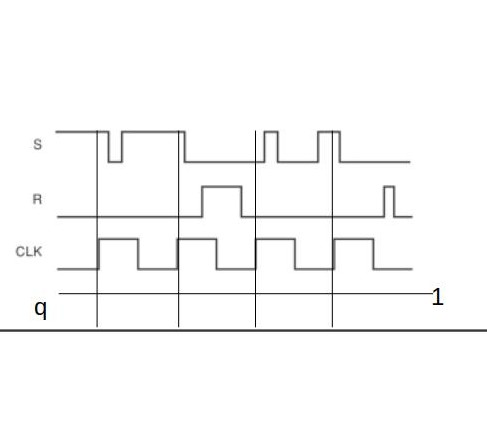
\includegraphics[scale = 0.3]{graph-3.jpg}\\
\begin{center}
	\begin{tabular}{|c|c|c|c|}		\hline
	S&R&CLK&Q\\
	\hline
	0&0&UP&$Q_0$\\
	\hline
	1&0&UP&1\\
	\hline
	0&1&UP&0\\
	\hline
	1&1&UP&Ambigous\\
	\hline 
	\end{tabular}
\end{center}

\problem{}{0}
\solution
\textcolor{blue}{}
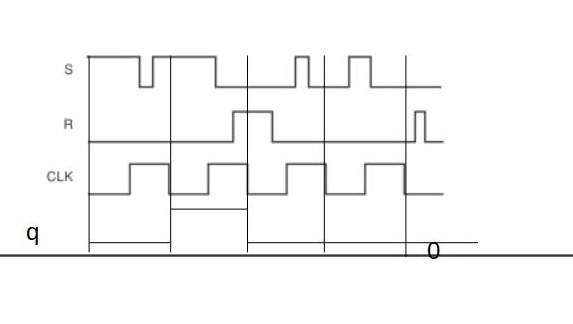
\includegraphics[scale = 0.3]{graph-4.jpg}
\begin{center}
	\begin{tabular}{|c|c|c|c|}		\hline
	S&R&CLK&Q\\
	\hline
	0&0&DOWN&$Q_0$\\
	\hline
	1&0&DOWN&1\\
	\hline
	0&1&DOWN&0\\
	\hline
	1&1&DOWN&Ambigous\\
	\hline 
	\end{tabular}
\end{center}

\problem{}{0}
\solution
\textcolor{blue}{}
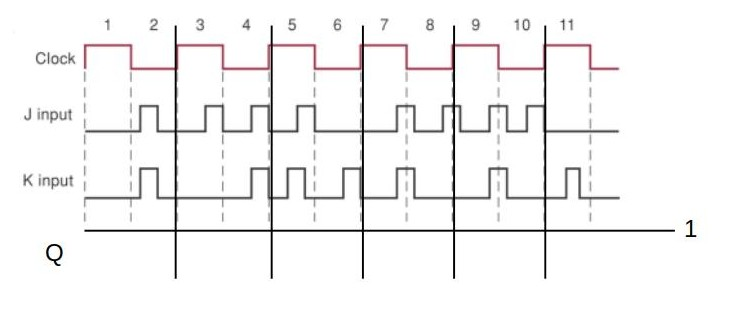
\includegraphics[scale = 0.3]{graph-5.jpg}
\begin{center}
	\begin{tabular}{|c|c|c|c|}		\hline
	S&R&CLK&Q\\
	\hline
	0&0&UP&$Q_0$(No change)\\
	\hline
	1&0&UP&1\\
	\hline
	0&1&UP&0\\
	\hline
	1&1&UP&$\overline{Q_0}$(toggles)\\
	\hline 
	\end{tabular}
\end{center}

\problem{}{0}
\solution
\textcolor{blue}{}
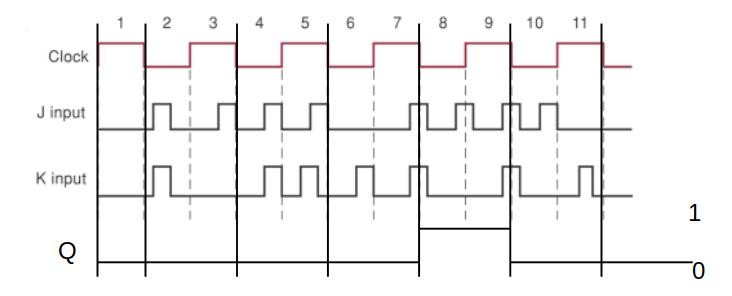
\includegraphics[scale = 0.3]{graph-6.jpg}
\begin{center}
	\begin{tabular}{|c|c|c|c|}		\hline
	J&K&CLK&Q\\
	\hline
	0&0&DOWN&$Q_0$(No change)\\
	\hline
	1&0&DOWN&1\\
	\hline
	0&1&DOWN&0\\
	\hline
	1&1&DOWN&$\overline{Q_0}$(toggles)\\
	\hline 
	\end{tabular}
\end{center}


\problem{}{0}
\solution
\textcolor{blue}{}
A) Let's start analyzing from the back. We want Y to get HIGH. We observe that it is a J-K flip flop, with grounded K. That means K = 0 for ever. Assuming the flip flop react on the positive going transitions, we want scenario where input J is HIGH, and timer to react after it, noticing the change. So what we want is J,C going high in this order. (According to state table from previous exercises). IN order J to get HIGH, we want X to get high. For that the situation is indentical, so we want to get A, then B HIGH, so we can register the change, and output HIGH at X, that will go to another J, and C will get HIGH, and after that Y will end up being high. So the order is A, B, C.\\
B)Since, the signal is connected to the CLR asynchrous input, it makes the X and Y outputs 0, it wipes it immideately.It is low input, so low start will set outputs to 0, "restarting" them. \\
C)
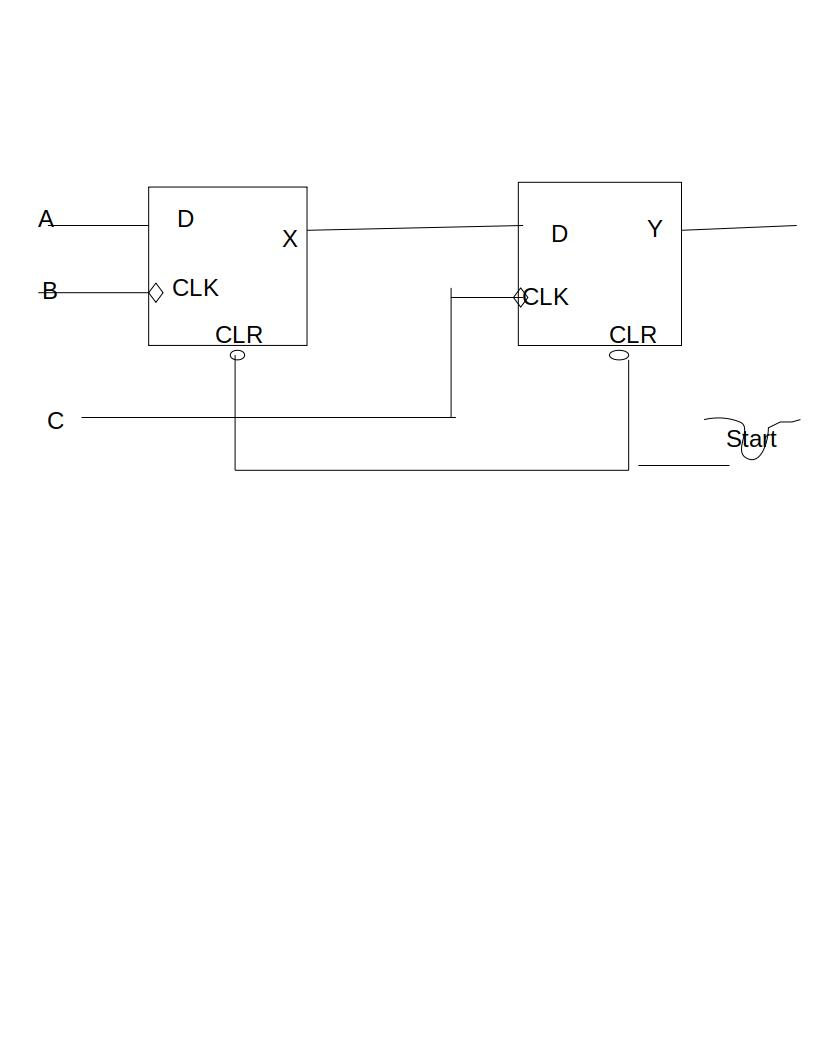
\includegraphics[scale=0.3]{circuit.jpg}
\end{document}